In the following, seven applications are presented to illustrate the versatility of \bioptim and give a practical overview on how to use its main features.
The \comment{performances}{Ajouter la RMS avec le single shooting} and the Github links of each OCP are summarized in Tab.~\ref{tab:Perfs_and_detailed_implementations_of_each_example}.


\subsection{Muscle activation driven pointing task}
%
\begin{figure}[t!]
\centering
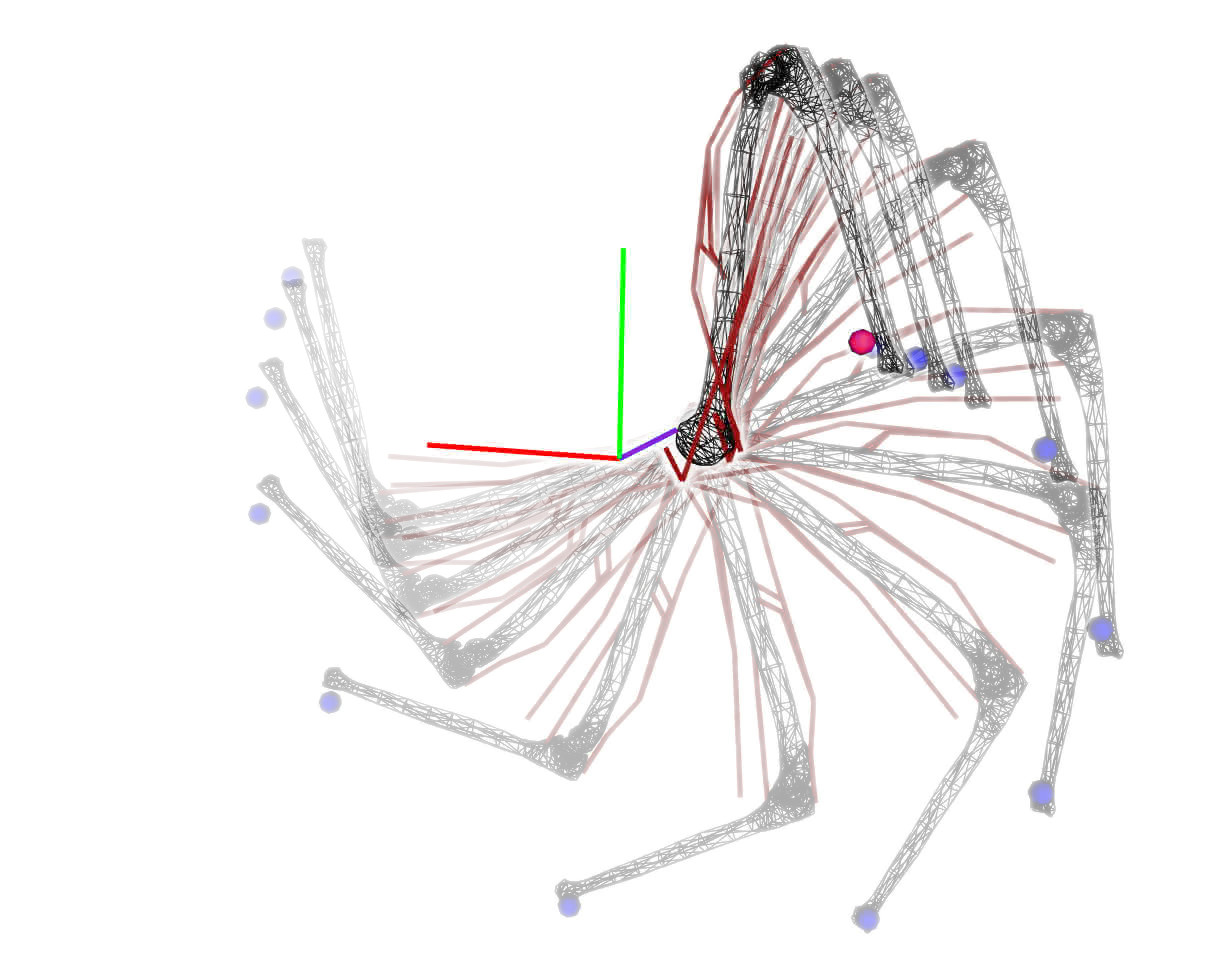
\includegraphics[width=\columnwidth]{figures/activation_pointing.jpeg}\\
\caption{Snapshots of an optimized activation-driven pointing task with \acados. The arm starts facing upwards in left hand part of the picture and ends facing downwards in the right hand part. The marker fized on the Ulna is depicted in blue and the scene-fixed target marker is depicted in red. Red lines show the lines of actions of the muscles.}
\label{fig:snapshots_activation_driven_pointing}
\end{figure}
\begin{figure*}[t!]
\centering
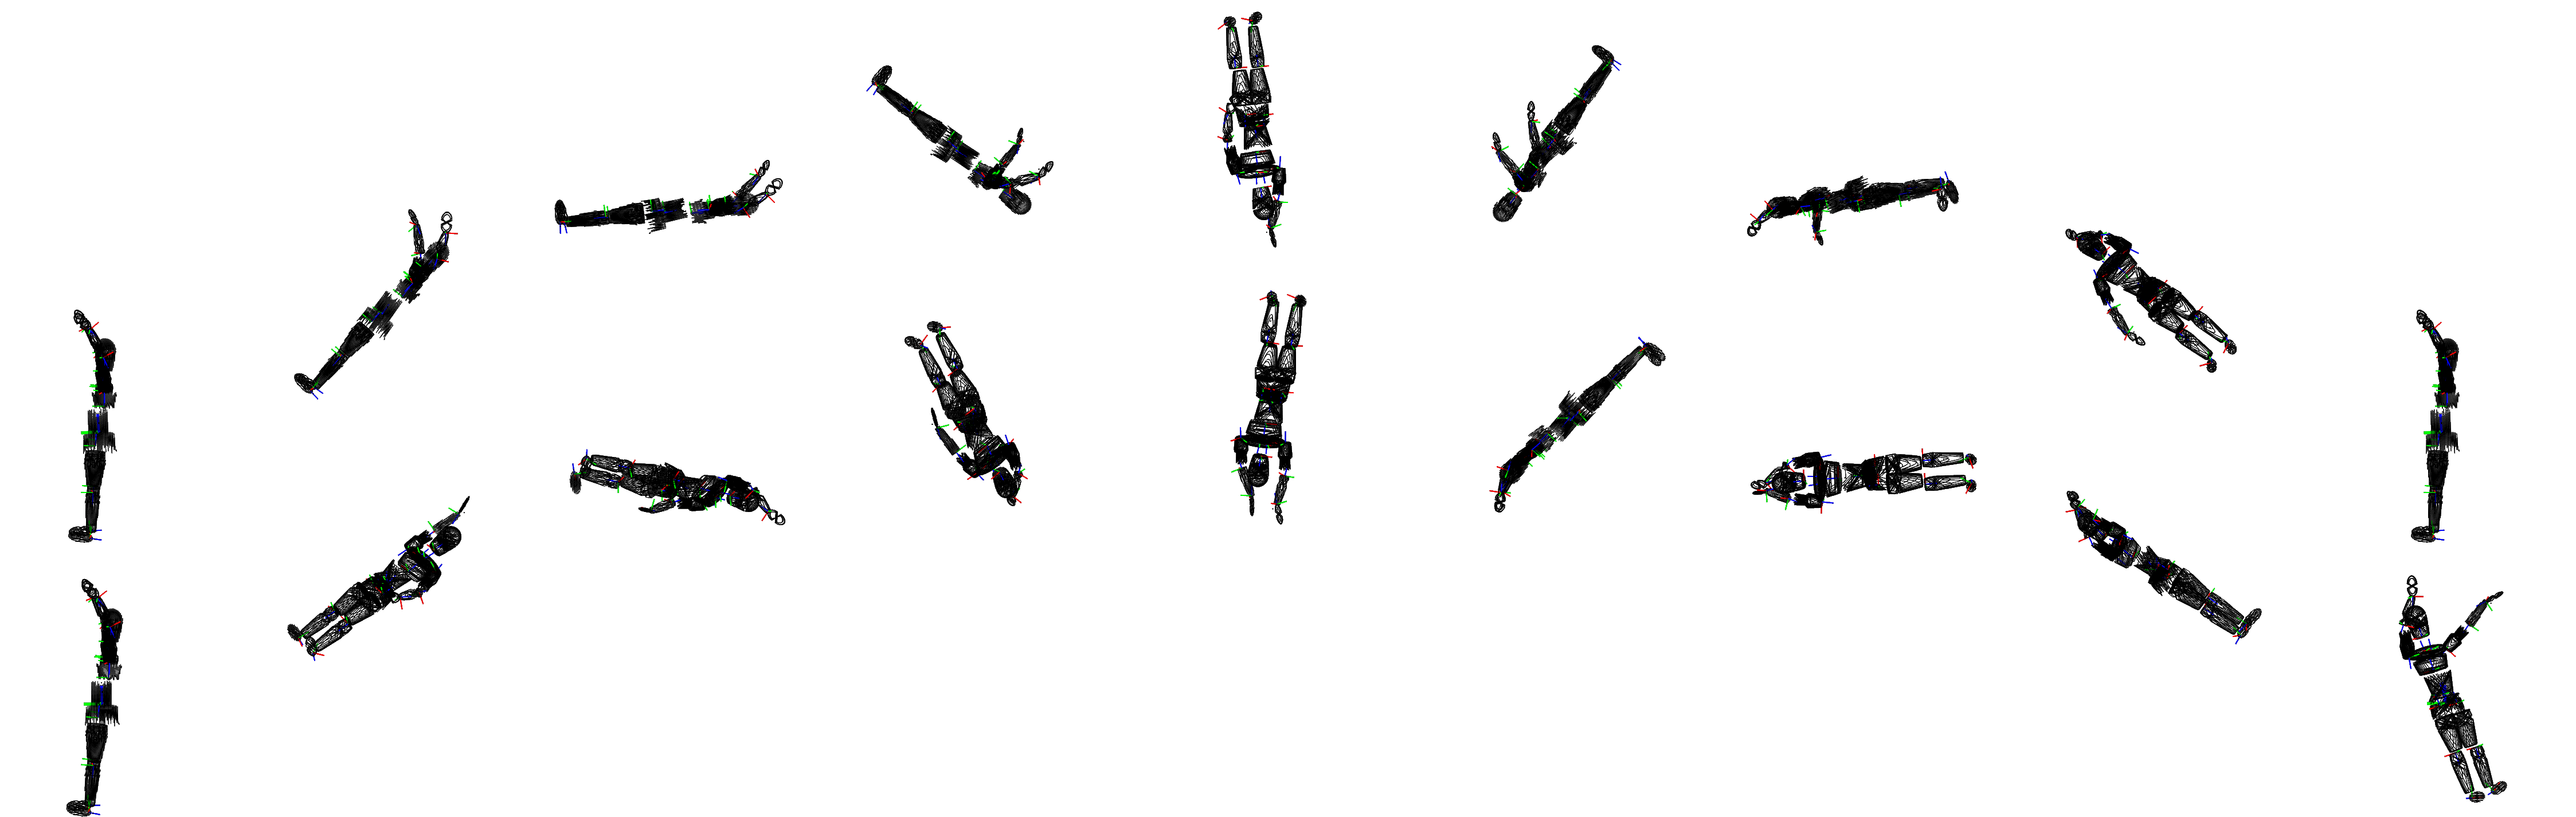
\includegraphics[width=\textwidth]{figures/Both_Bioptim_MaxVrille.png}
\caption{Snapshots of maximally twisting somersaults driven by shoulder torque actuators and a free base whose rotation is either expressed by Euler angles (top) or by quaternions (bottom).}
\label{fig:snapshots_quaternion_base_twisting_somersault}
\end{figure*}
%
In this first example, the goal was to achieve a muscle activation driven pointing task using a 2-DoF arm model with 6 muscle elements. 
In addition to muscle-induced torques, pure joint torques were added to compensate for the model weaknesses.
The main term (highest weight) of the objective function (Eq.~\ref{eq:cost_pointing}) is a Mayer objective, corresponding to the pointing tasks at the final node, to superimpose two markers, the first one, $\mathbf{m_u}$, fixed in the Ulna system of coordinates and the second one, $\mathbf{m^*_s}$, fixed in the scene.
The three Lagrange terms  were added for control regularization (muscle activation $\bf{a}$ and joint torques $\boldsymbol{\tau}$) and for state ($\bf{x}$) regularization:
\[
\begin{aligned}
	\mathcal{C} = 	&~\omega_1~\underbrace{\|\mathbf{m_u}(T)-\mathbf{m^*_s}\|^2}_{\mathtt{TRACK\_MARKERS}}~\\
	&\int_{t=0}^T\underbrace{\|\bf{a}\|^2}_{\mathtt{MIN\_ACTIVATION}}~
	+\underbrace{\|\boldsymbol\tau\|^2}_{\mathtt{MIN\_TORQUE}}~
	+\underbrace{\|\bf{x}\|^2}_{\mathtt{MIN\_STATE}}~ dt,
\end{aligned}
\addtag
\label{eq:cost_pointing}
\]

\noindent where T is the duration of the motion, and $\omega_1=1e5$.
The movement lasted for 2~seconds and was discretized using 50~shooting nodes with a 5-steps RK4 integration in-between.
The problem was solved using \ipopt (with exact Hessian computations) and \acados (with a Gauss-Newton approximation of the Hessian) resulting in two very close solutions.
\acados was about 50 times faster than \ipopt and was better at enforcing the continuity constraints (as shown by the single shooting error in Tab.~\ref{tab:Perfs_and_detailed_implementations_of_each_example}).
\ipopt however ended up with a smaller optimized objective (20.8 \textit{vs} 23.2), leading to a more optimal solution than \acados. 
Superimposed snapshots of the optimal motion found with \acados are displayed in Fig.~\ref{fig:snapshots_activation_driven_pointing}.
It is worth mentioning that for the purpose of this illustration, no constraint was given on the shoulder range of motion to ensure physiological muscle trajectories. 










\subsection{Quaternion base twisting somersault}
The goal was to maximize the twist rotation ($\phi$) in a backward somersault.
The model is composed of a 6-DoF root segment and two 1-DoF torque actuated arms.
The OCP was solved for two models.
First, rotations of the root segment were expressed as Euler angles.
They were expressed as a quaternion for the second model.
The objective functions were written as follow:

\begin{eqnarray}\label{eq:ocp_Trampo}
\mathcal{J} = -\underbrace{\int_0^T \dot{\phi}~dt}_{MINIMIZE\_TWIST}  +~\omega_1 \underbrace{\int_0^T \sum_{i=1}^{2}~\tau_{i}^2~dt}_{MINIMIZE\_ TORQUE},
\end{eqnarray}
with $\omega_1 = 1\times 10^{-6}$, T the duration of the movement and $\tau_{i}$ the torque control of the $i^{th}$ arm DoF.
The first term of the objective function (Eq.~\ref{eq:ocp_Trampo}) corresponds to maximizing the twist velocity and the second term is for control regularization.


The movement lasted for approximately 1 second and was discretized in 100 shooting nodes.
The solutions for both models were similar (Fig.~\ref{snapshots_quaternion_base_twisting_somersault}) highlighting the equivalence of the two rotation representations.
Euler angles have the advantage to be easily interpretable, but they suffer from the loss of a DoF at the gimbal lock.
The use of quaternion representation is advantageous for numerical stability when a joint is free to rotate on a wide three-dimensional range for motion.


\begin{figure*}[t!]
\centering
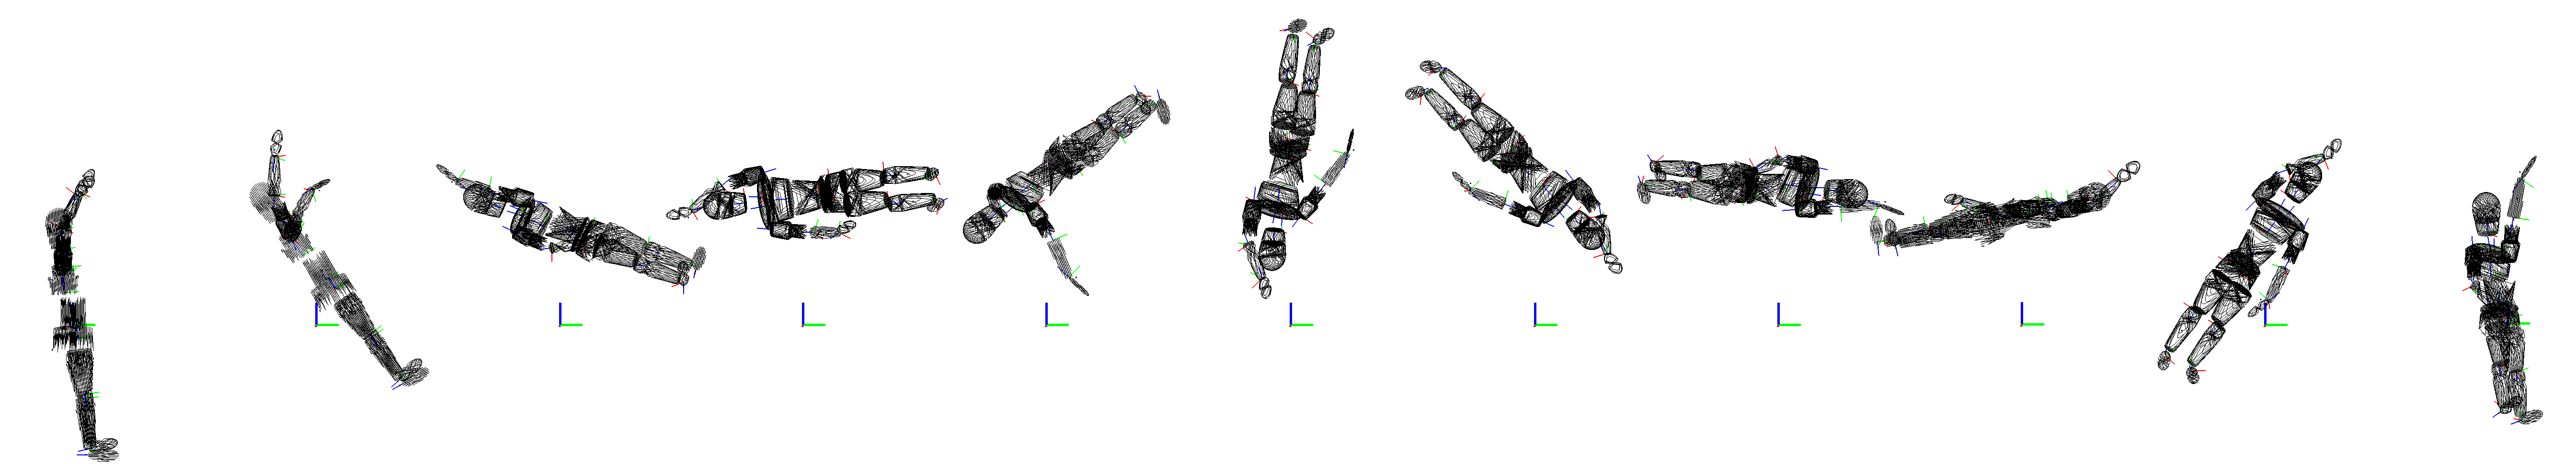
\includegraphics[width=\textwidth]{figures/Euler_Bioptim_MaxVrille_2.png}\\
\vspace*{0.5em}
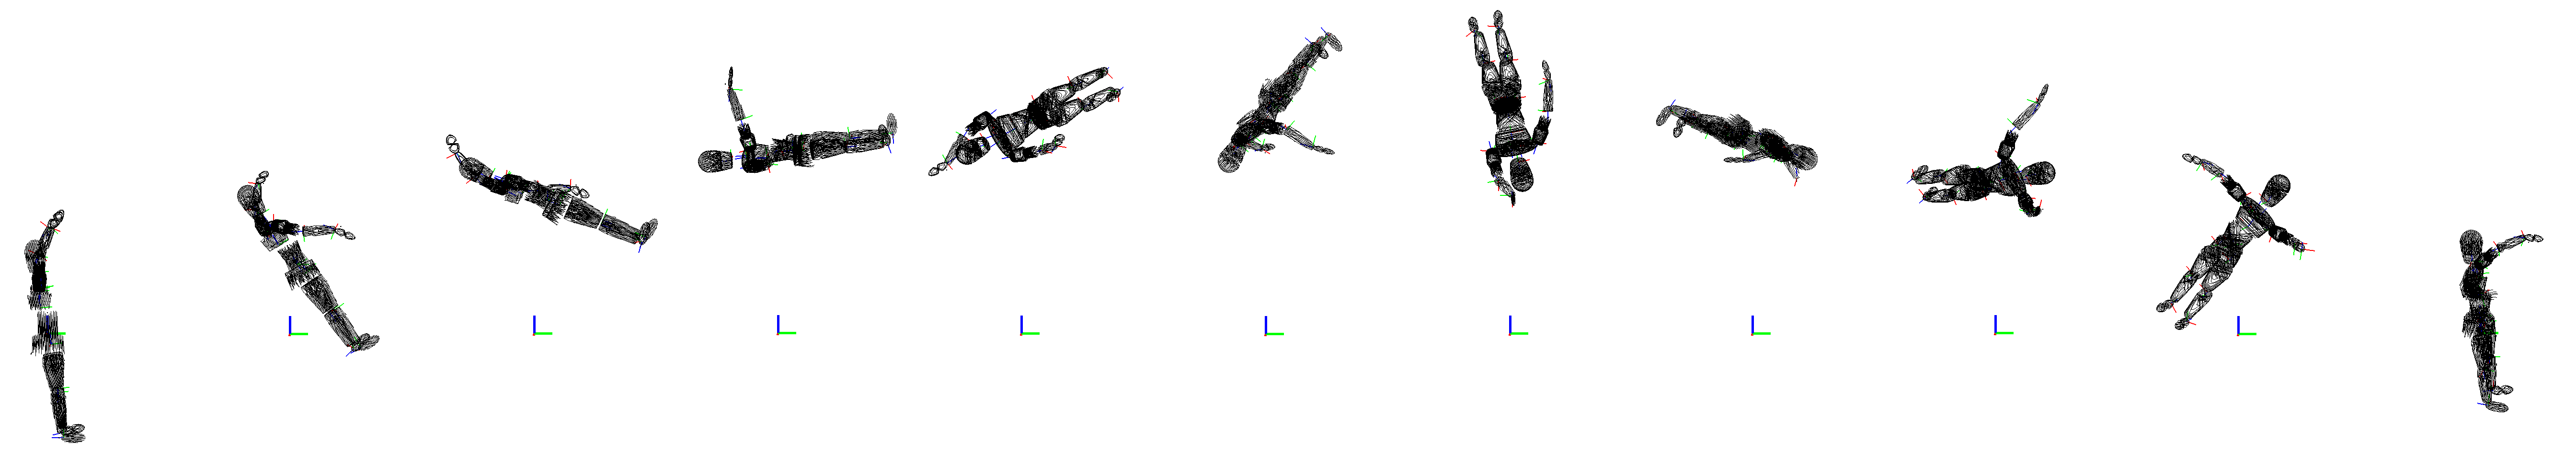
\includegraphics[width=\textwidth]{figures/Quat_Bioptim_MaxVrille_2.png}
\caption{Snapshots of a maximally twisting somersault driven by shoulder torque actuators and a free base expressed by Euler angles (top) or quaternions (bottom).}
\label{fig:snapshots_quaternion_base_twisting_somersault}
\end{figure*}


% \begin{table}[h!]
% \caption{\small Objective terms of quaternion base maximally twisting somersault}
% \label{tab:Quaternion_base_twisting_somersault}
% \centering
% \begin{tabular}{c c c c}
% \toprule 
% & Type & Function & Weight \\ 
% \midrule
% $\#1$ & Lagrange & MINIMIZE\_TWIST & $-1e1$ \\ 
% \midrule
% $\#2$ & Lagrange & MINIMIZE\_ TORQUE & $1e-6$ \\ 
% \bottomrule
% \end{tabular}
% \end{table}















\subsection{Pendulum on a spring}
This spring-mass-pendulum-based example is presented to introduce \textit{bioptim}'s ability to use of external forces.
The goal was to maintain the position of a $\SI{1}{kg}$ mass hanging on a linear spring attached to the ground.
A $\SI{0.2}{m}$-long pendulum weighting $\SI{10}{kg}$ was attached to the mass and free to rotate in one dimension (Fig.~\ref{fig:Mass_Pendulum_Model}).
In addition to the spring force, the mass was actuated by a vertical force (e.g., somebody pulling on it) while the pendulum rotation was passive.
The system therefore comprised two DoFs, the mass position ($q_m$) and the pendulum angle ($q_p$) and one control input, the vertical force pulling on the mass ($f$). 
\begin{figure}[h!]
\centering
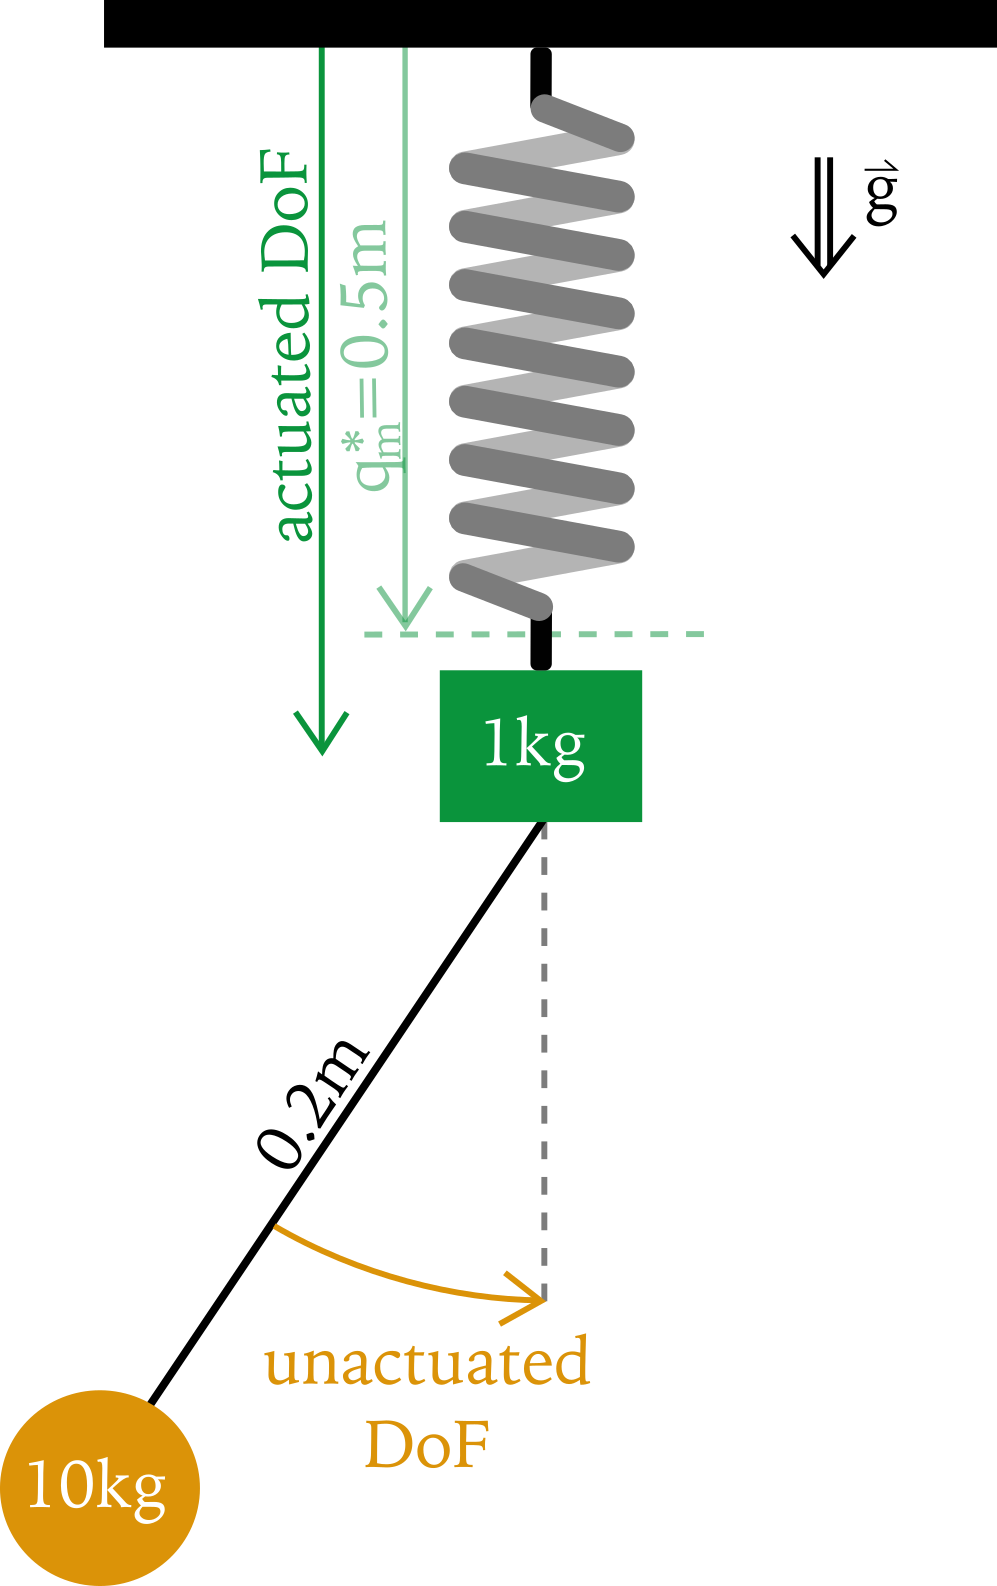
\includegraphics[width=0.35\columnwidth]{figures/Mass_Pendulum_Model.png}
\caption{Definition of the spring-mass-pendulum model.}
\label{fig:Mass_Pendulum_Model}
\end{figure}
The spring force $f_s$ was:
\[
\begin{aligned}
f_s = -k*q_m,
\end{aligned}
\addtag
\label{eq:f_ext}
\]
with k the spring stiffness constant.\\
The OCP was composed of two phases each lasting for $\SI{5}{s}$, with 50 shooting nodes.
In the first phase, no objective function was minimized and $f$ was constrained to $0$ letting the mass oscillating freely. 
Then, in the second phase, a cost function (Eq.\ref{eq:ocp_Pendulum}) was minimized, to enforce a specific position for the mass.
Theis objective function, exclusively composed of Lagrange terms, was formulated as follow:
\[
\mathcal{J} = \underbrace{\int_{T/2}^T (q_m - q_m^*)^2~dt}_{\mathtt{TRACK\_STATE}}  +~\omega_1 \underbrace{\int_{T/2}^T ~\tau^2~dt}_{\mathtt{MIN\_ TORQUE}},
\addtag
\label{eq:ocp_Pendulum}
\]

\noindent with $q_m$ and $q_m^* = -0.5m$ respectively the optimized and reference positions of the mass, $\omega_1 = 1\times 10^{-6}$, T the duration of the movement and $\tau$ the force control of the mass.
The first term of the objective function (Eq.~\ref{eq:ocp_Pendulum}) acts as a position controller for the mass.
The second as added for control regularization.


During the first phase, the mass is oscillating passively around it's stationary position due to the force exerted by the spring.
However, when the mass gain the ability to react actively with force actuation, it stabilizes around the targeted position (Fig.~\ref{fig:Mass_Pendulum_Fext_graphs}).
This example highlights the possibility of using optimal control to find activation patterns compensating for external passive forces (e.g., ortheses flexibility, contact surface deformation, interaction between two models, ...).

\begin{figure*}[t!]
\centering
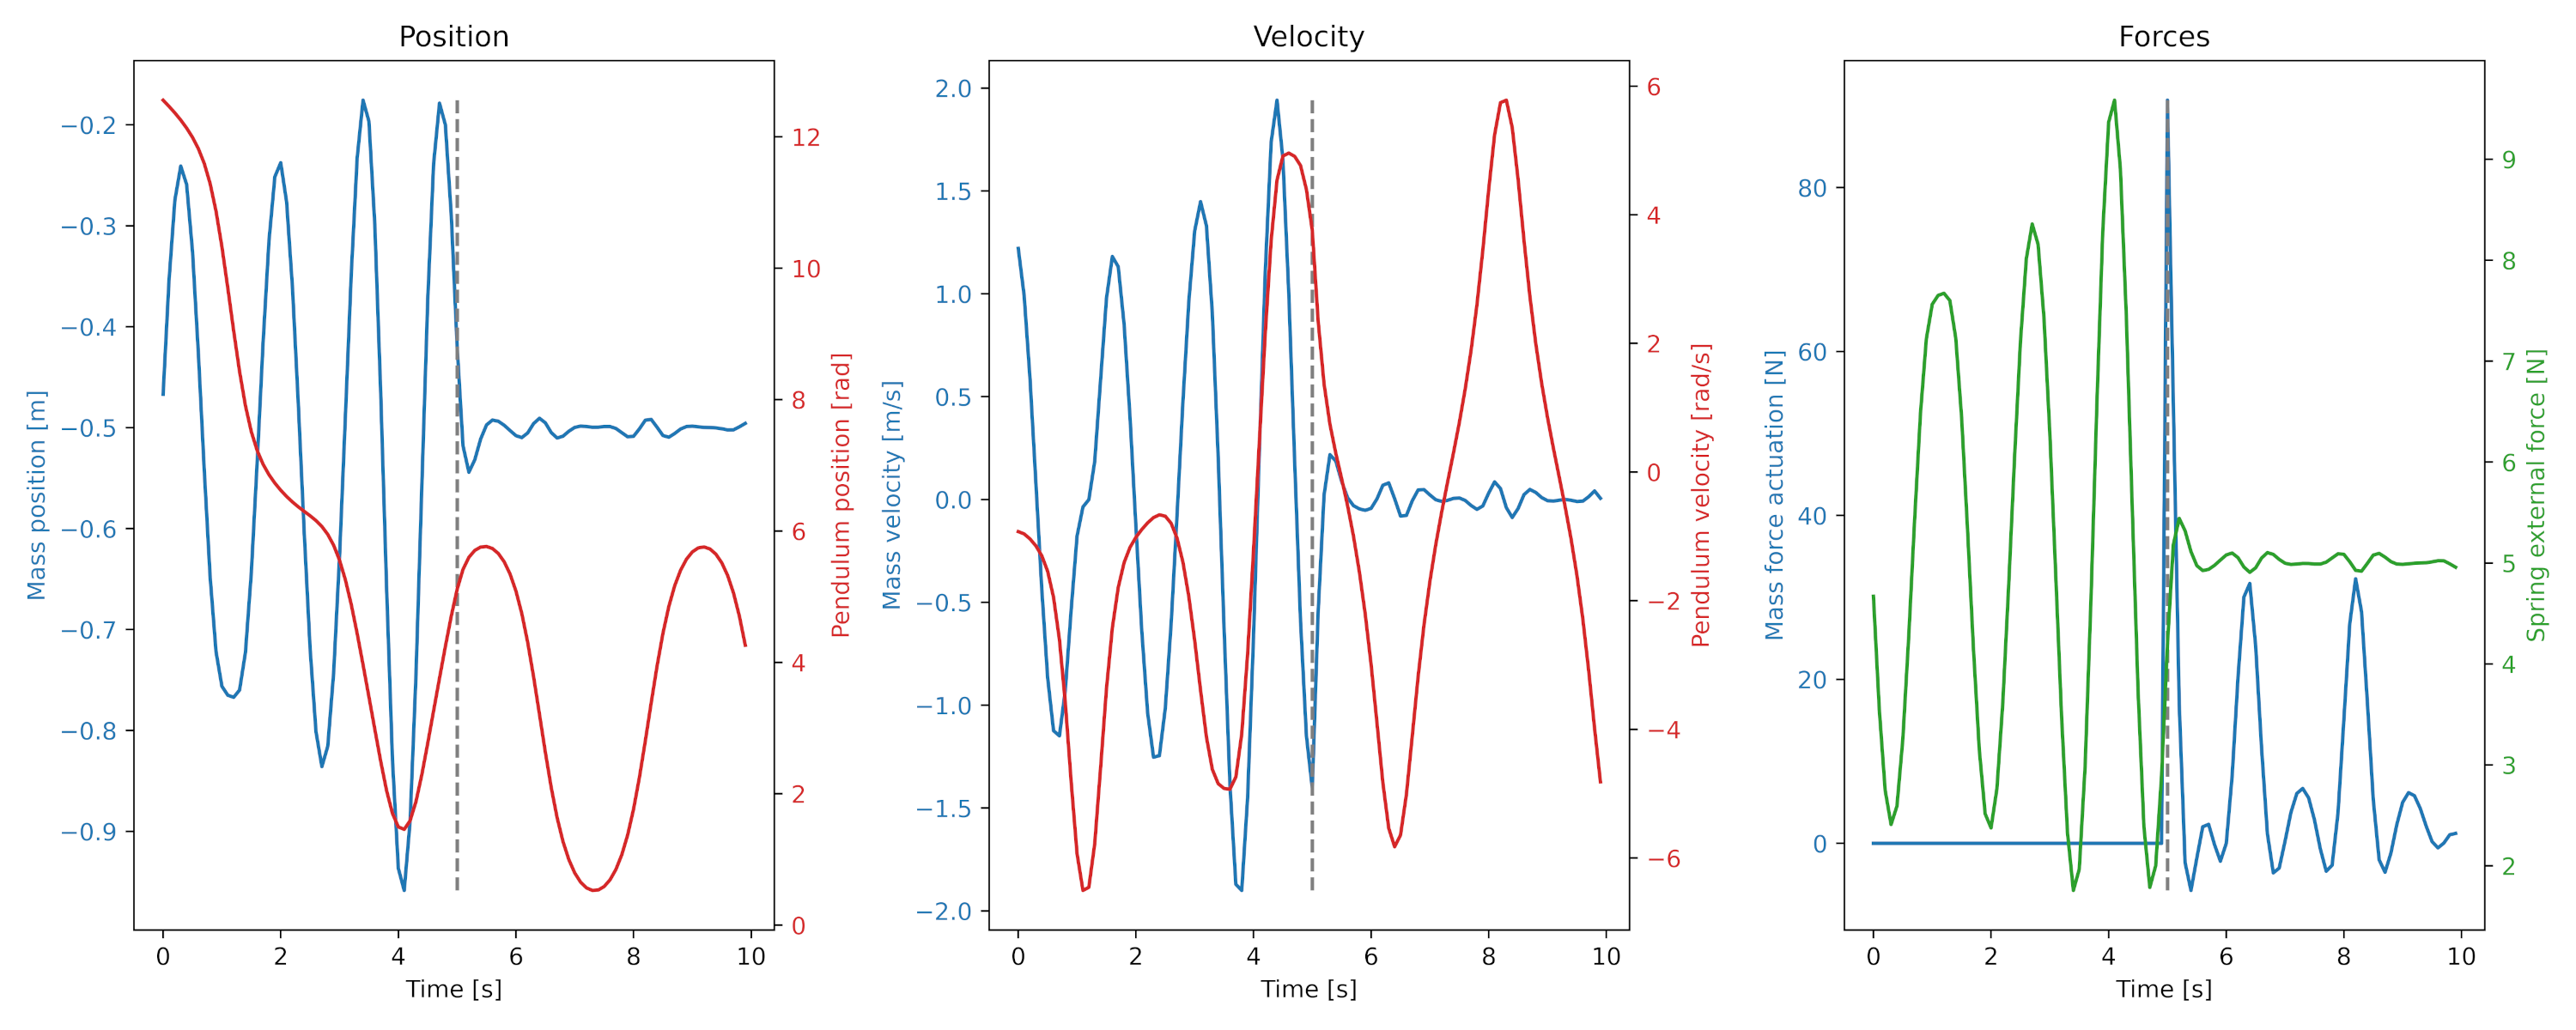
\includegraphics[width=\textwidth]{figures/Mass_Pendulum_Fext.png}
\caption{Optimal kinematics of the mass-pendulum-spring system. Gray dashed lines show the stage transition, blue lines are related to the mass, red lines are related to the pendulum and the green line is related to the spring.}
\label{fig:Mass_Pendulum_Fext_graphs}
\end{figure*}
















\subsection{Multiphase torque driven walking cycle}
This example is presented to introduce \textit{bioptim}'s ability to deal with a multiphase locomotion estimation problem with muscle actuation and contact forces.
The goal was to estimate muscles activation by tracking markers trajectories and ground reaction forces and moments. 
The model was a 3D leg with 12 DoFs (6-DoFs pelvis, 3-DoFs hip, 1-DoF knee and 2-DoFs ankle), driven by 17 muscle activations and residual joint torques to compensate for potential muscle actuation weaknesses. 
The gait cycle was defined from the first heel strike to the end of the swing phase discretized into 90 shooting intervals. 
To follow the natural rolling of the foot, the stance was divided into three phases (heel, flatfoot and forefoot contacts) of fixed duration deduced from experimental force platform data and markers position ($0.05$, $0.36$ and $0.16$\:s).
The swing phase lasted $0.38$\:s. 
The interaction between the ground and the foot was modeled using a 4-contact points model located at the heel and the forefoot (first, fifth metatarsi and hallux).
The optimization problem consisted in minimizing the errors between predicted $\bf{m}$ and reference $\bf{m}^*$ markers trajectories, predicted $\bm{\mathcal{F}}$, $\bm{\mathcal{M}}$ and reference $\bm{\mathcal{F}^*}$, $\bm{\mathcal{M}}^*$, respectively ground reaction forces and moments at all contact points.
$^*$ stands for reference (i.e., measured) data.
A regularization term on muscle activations, $\bf{a}$, was also added (least-activations) as well as a penalization term on the residual torques $\boldsymbol{\tau}$:

\[ 
\resizebox{0.9\columnwidth}{!}{$ 
\begin{aligned}
%\mathcal{J} = &\int_{t=0}^{T}\underbrace{\omega_1(\|m_p - m_m\|^{2})}_{\mathtt{TRACK\_MARKERS}}~ 
%+ ~ \underbrace{\omega_2(\|f_p - f_c\|^{2})}_{\mathtt{TRACK\_FORCES}}\\
%&+ ~ \underbrace{\omega_3(\|tau^f_p - tau^f_m\|^{2})}_{\mathtt{TRACK\_MOMENTS}}~
\mathcal{J} = &\int_{t=0}^{T}\underbrace{\omega_1(\|\bm{m} - \bm{m}^*\|^{2})}_{\mathtt{TRACK\_MARKERS}}~ 
+ ~ \underbrace{\omega_2(\|\bm{\mathcal{F}} - \bm{\mathcal{F}}^*\|^{2})}_{\mathtt{TRACK\_FORCES}}\\
&+ ~ \underbrace{\omega_3(\|\bm{\mathcal{M}} - \bm{\mathcal{M}}^*\|^{2})}_{\mathtt{TRACK\_MOMENTS}}~
+ ~ \underbrace{\omega_4\|\bf{a}\|^2}_{\mathtt{MIN\_ACTIVATION}}
+ ~ \underbrace{\|\boldsymbol{\tau}\|^2}_{\mathtt{MIN\_TORQUE}}~dt, 
\end{aligned}  
$}  
\addtag  
\label{eq:ocp_walk}  
\]

\noindent where $\omega_1$=1e5, $\omega_2$=0.1, $\omega_3$=0.1, $\omega_4$=10 are  weighting factors and $T$ is the the duration of the current phase.\\

Non-slipping ($\mathtt{NON\_SLIPPING}$) and unilateral contact force ($\mathtt{CONTACT\_FORCE}$) constraints were added to prevent the foot from slipping and pulling from the ground. 
In between phases, the use of the $\mathtt{IMPACT}$ state transition allowed to represent the gain or loss of contact(s) in the dynamics (e.g., swing phase to heel strike [Felis (2016)]) \\
% ~\cite{felis_2016_contact}[Felis (2016). Synthesis of Full-Body 3-D Human Gait using Optimal Control Methods. doi:10.1109/ICRA.2016.7487294]

Tracking experimental data allowed to reproduce leg motion during the walking cycle (Fig.~\ref{fig:snapshots_multiphase_walking_cycle}). 
The root mean square tracking error on markers trajectories was $27$ mm (mean error on pelvic and foot markers was $7.5$ mm and $14.7$ mm, respectively). 
Concerning ground reaction forces tracking, the root mean square error was $4.85$ N.
Gluteal muscles were mainly activated during the stance and with a significant activity during the swing phase (Fig.~\ref{fig:muscles_activation_gait} for all activations). 
The Gluteus Maximus was mainly activated during the early flatfoot phase with a maximal activation of $0.2$ allowing to prepare the stance phase. 
For the thigh muscles, the semimembranous, semitendinous and biceps femoris were activated during the early stance phase and terminal swing (maximal activation of $0.3$, $0.4$ and $0.4$, respectively). 
Those results were similar to the characteristic average activity patterns of the lower limb muscles during locomotion described by Winter (1991). 
% ~\cite{winter_1991} [Winter DA (1991). The Biomechanics and Motor Control of Human Gait: Normal, Elderly and Pathological.]
The knee extensors, vastus lateralis, medialis and intermedius followed the same pattern and were mainly activated during the flatfoot phase (ie loading response).
However, the highest activity of the rectus femoris appeared at forefoot phase (terminal stance) and pre swing.
Leg muscles were highly activated (saturation of gastocnemius lateralis and medialis) at the terminal stance and early swing. The tibialis anterior is the sole muscle for dorsiflexion and the only antagonist of the triceps surae in this model which could explain its high activity at the same time. 

\begin{figure*}[t!]
\centering
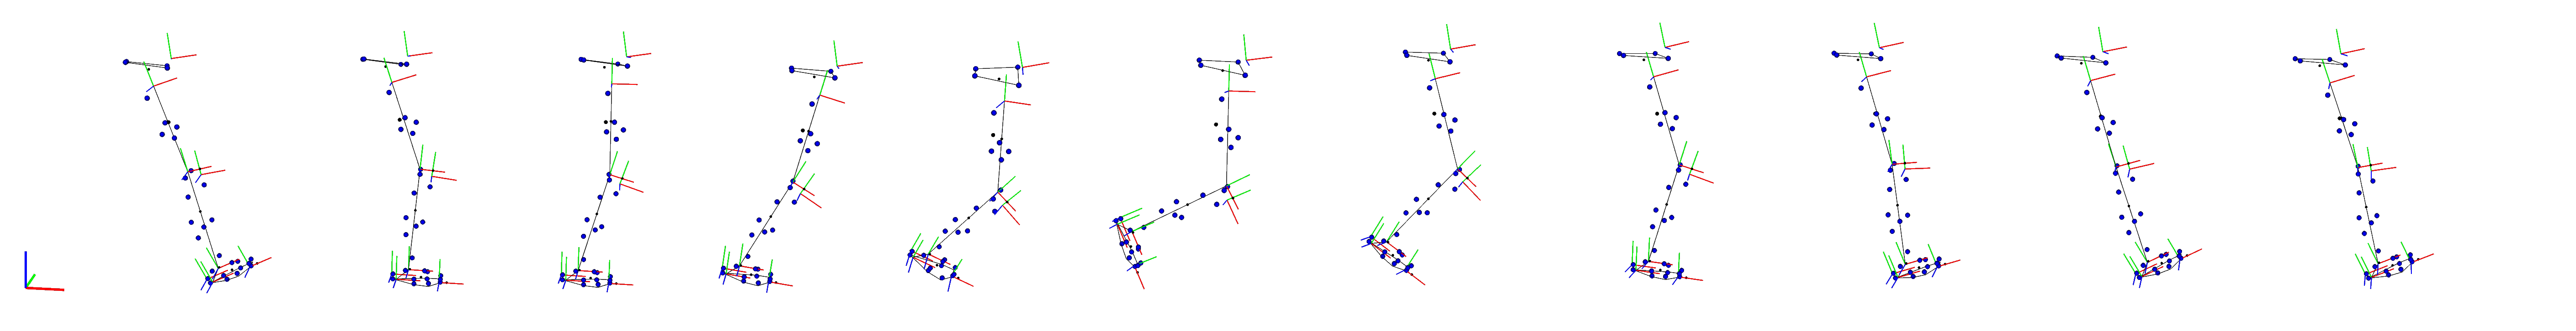
\includegraphics[width=\textwidth]{figures/multiphase_walking_cycle.png}\\
\caption{Snapshots of a walking gait cycle driven by muscles activation.}
\label{fig:snapshots_multiphase_walking_cycle}
\end{figure*}

\begin{figure*}[t!]
\centering
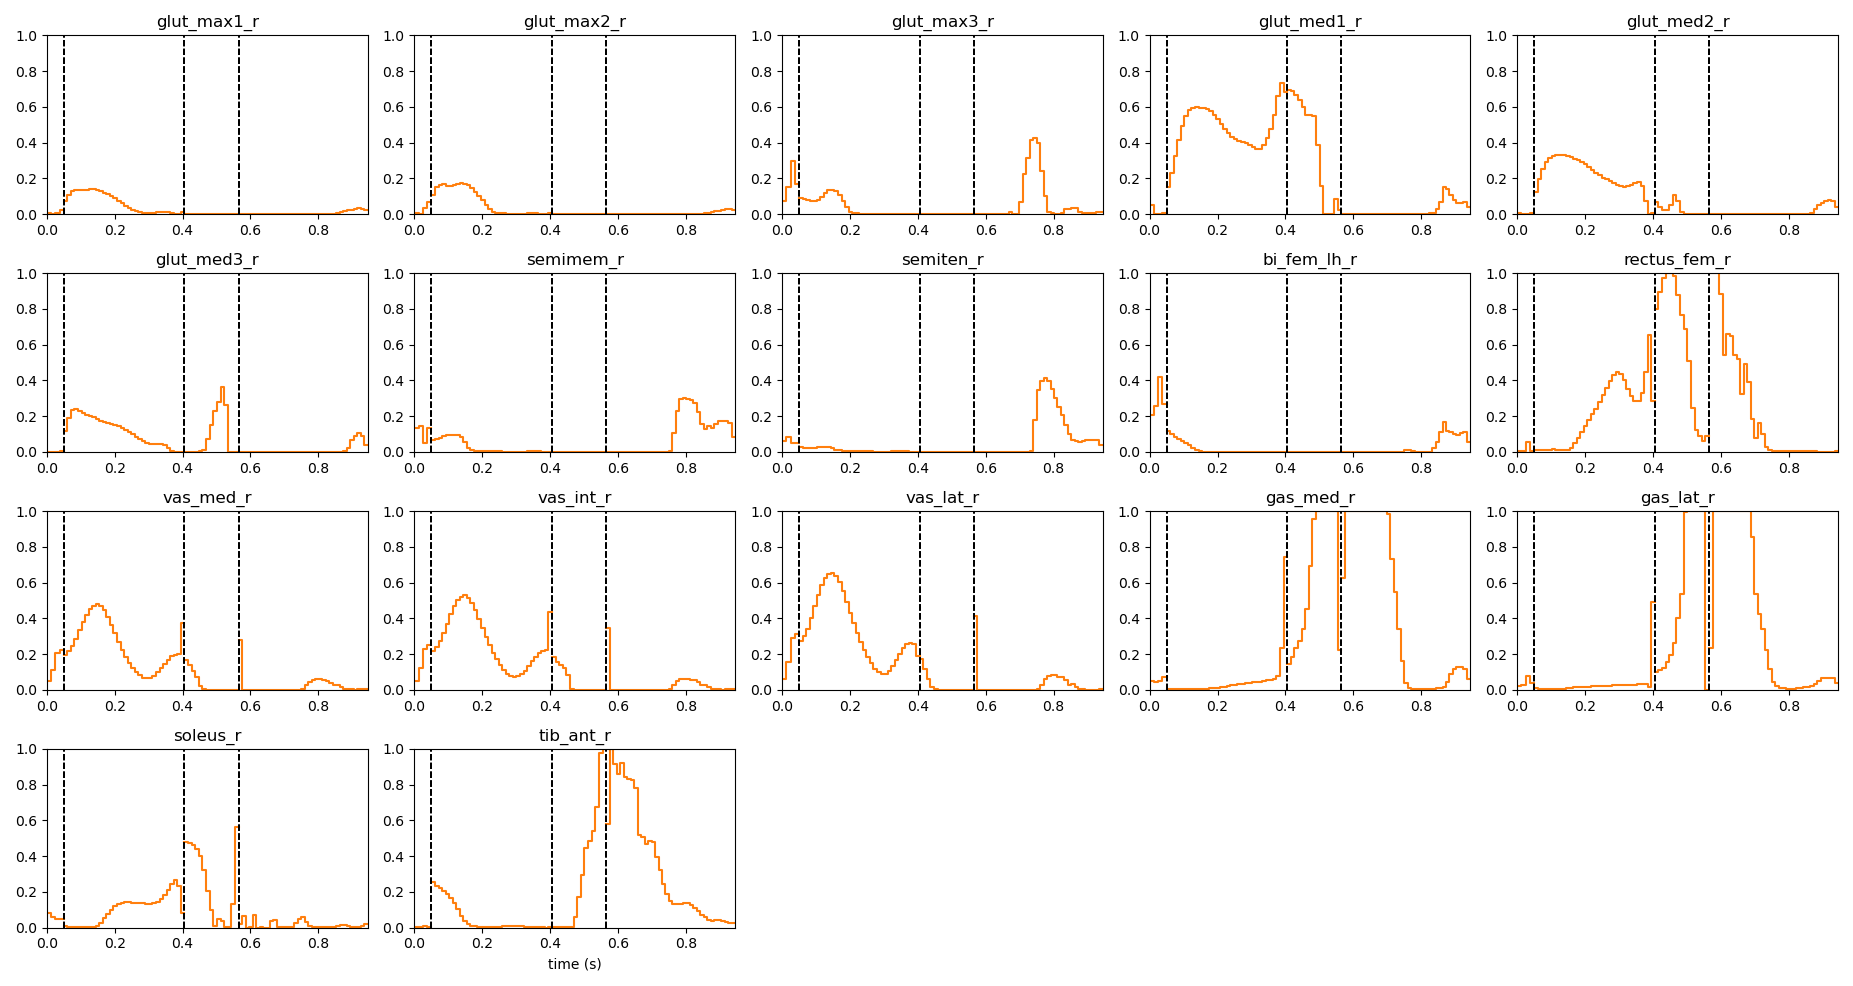
\includegraphics[width=\textwidth]{figures/muscles_control_gait_example.png}\\
\caption{Muscle activity patterns during walking cycle.}
\label{fig:muscles_activation_gait}
\end{figure*}


\subsection{Moving Horizon Estimation of Shoulder Elevation}
This example is presented to introduce \bioptim's ability to provide real-time estimation of biomechanical variables.
The goal was to perform a real-time estimation of dynamically consistent joint kinematics and muscle forces, using a moving horizon estimation (MHE) approach (i.e. an optimization approach that uses a series of measurements observed over time). 
A shoulder elevation motion was performed with a 4-DoFs ($\bf{q}$) arm actuated by 19 Hill-type muscle elements.
The control inputs of the model were the muscle activations ($\bf{a}$).
The MHE implementation consists in splitting the OCP into a succession of smaller one for processing fixed-size subsets of the tracking data moving forward in time. 
Each time one subproblem is solved, a new measurement is added, the oldest one is discarded and a new subproblem is defined. 
Due to their similarities, the solution of the previous OCP is a good initial guess to the new one. 
The dynamical consistency of the final solution is enforced by continuity constraints on the initial state. 
Each objective function (Eq.~\ref{eq:ocp_exMHE}) was written as the sum of three terms: tracking reference joint angles ($\bf{q^*}$), states and muscle activations regularizations (i.e., least-square criteria): 
\begin{figure}[t!]
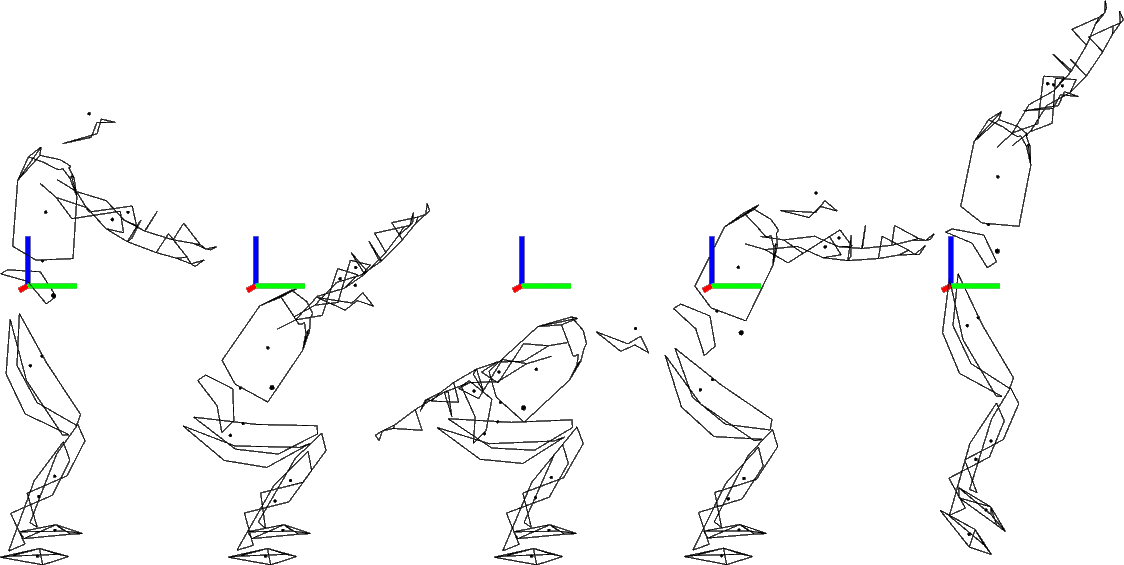
\includegraphics[width=\columnwidth]{figures/kinogramme_jump}
\caption{Snapshots of the push-off phase of a vertical jump (Ex.~\ref{ex:jump}). The avatar reproduces a human-like jump movement. The first four positions represent the first phase of the optimization (i.e., heel and toe in contact with the floor) and the fifth position depicts the end of the second phase (i.e., only the heel in contact with the floor)} 
\label{fig:graph_force_vitesse_longueur}
\end{figure}
\begin{figure*}[t!] 
\centering 
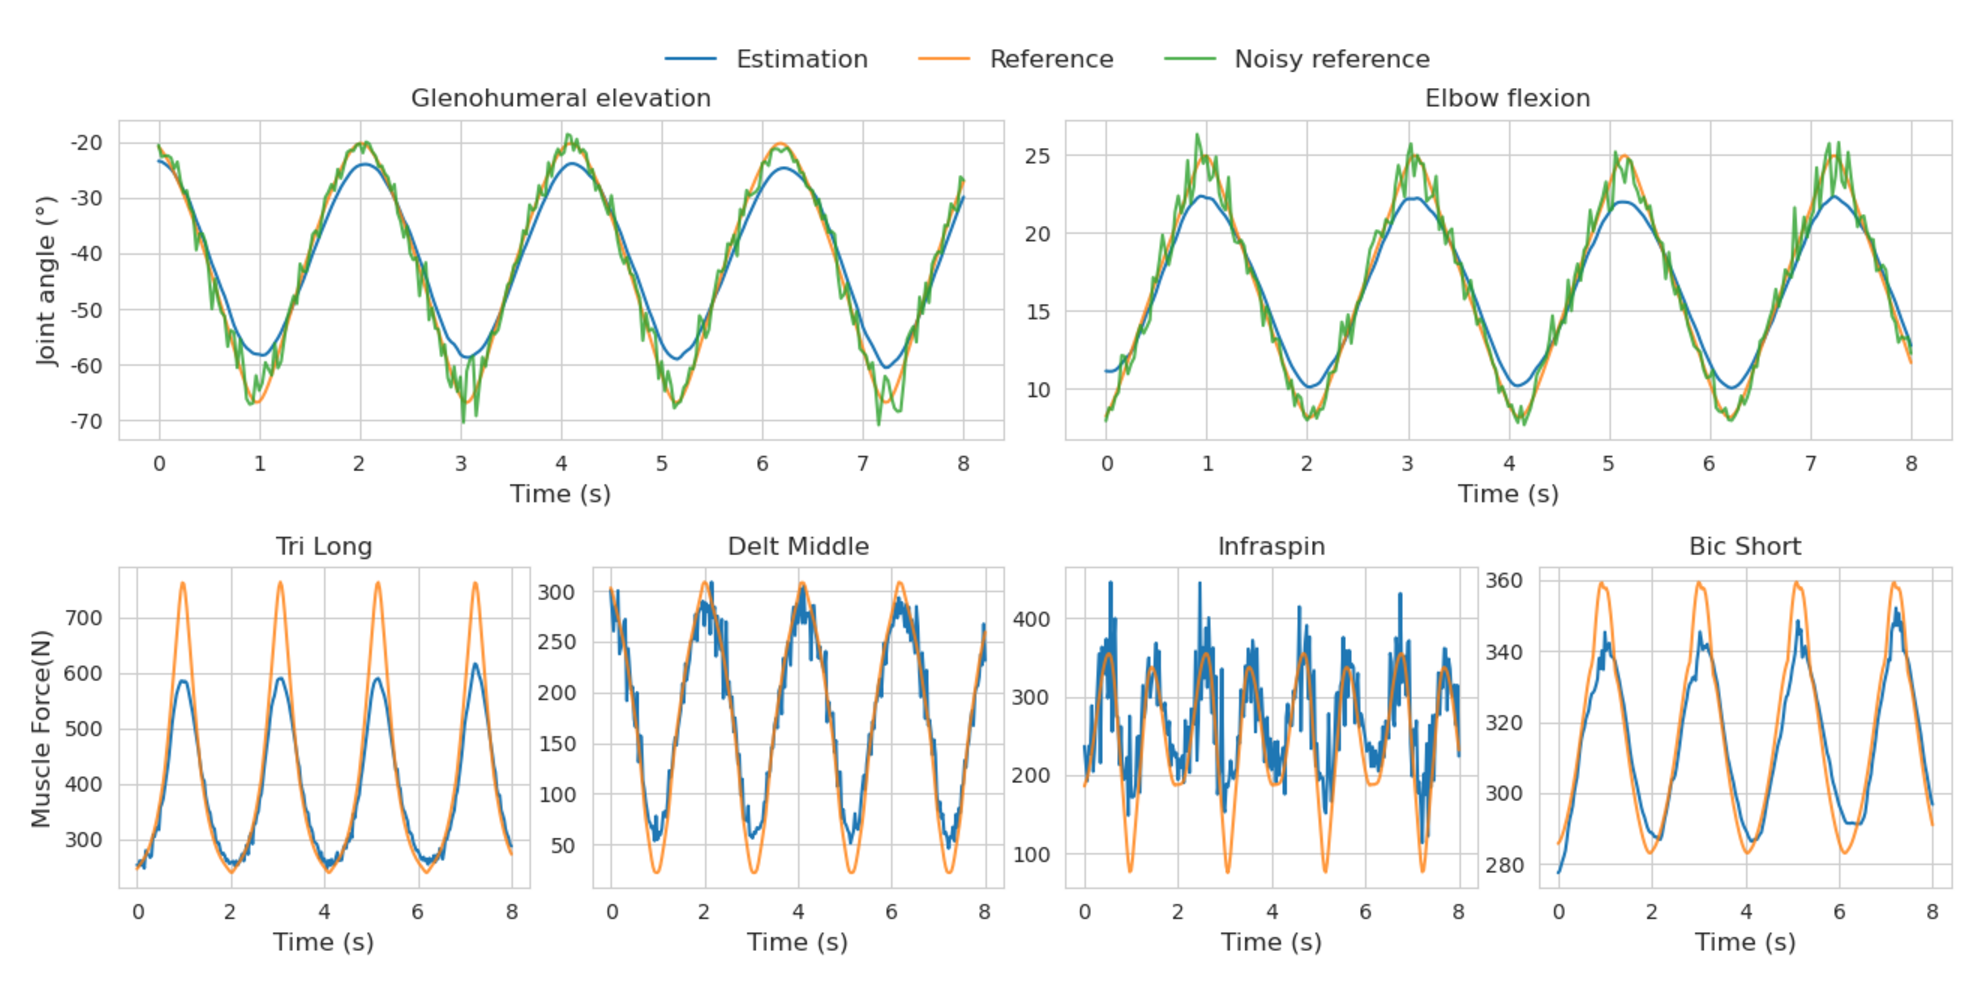
\includegraphics[width=\textwidth]{figures/MHE_results.pdf}\\
\caption{Time series of (1) real-time estimated joint angles (blue), reference joint angle (orange) and noisy reference joint angles (green) of a cyclic motion (up).
(2) Real-time estimated muscle forces (blue) and ground truth muscle forces (orange) of a cyclic motion (bottom) (Ex.~\ref{ex:mhe}).
Only four muscles with significative action (peaks force $>$ 15~N), on the two selected DoFs, are shown.
Muscle abbreviations stand for (from left to right): Triceps Long head, Deltoid Middle, Infraspinatus, Biceps Brachial Short head. (Ex.~\ref{ex:mhe}).} 
\label{fig:MHE_results}
\end{figure*} 
\\ 
\[ 
\resizebox{0.9\columnwidth}{!}{$ 
\begin{aligned}
\mathcal{J} = &\int_t^{t+t_{mhe}}\underbrace{\omega_1´(\|\boldsymbol{q} - \boldsymbol{q^*}\|^{2})}_{\mathtt{TRACK\_STATE}}~ 
+ ~ \underbrace{\omega_2\|\boldsymbol{q\|^2}}_{\mathtt{MIN\_STATE}} 
+ ~ \underbrace{\omega_3\|\boldsymbol{a\|^2}}_{\mathtt{MIN\_ACTIVATION}}~dt, 
\end{aligned}   
$}  
\addtag  
\label{eq:ocp_exMHE}  
\]  

\noindent where $\omega_1 =10^3$, $\omega_2 = 10$, $\omega_3 = 10^2$ and $t_{mhe}$ is duration of each sub-problem. 

In this example, reference data of an $8~s$ series of four arm elevations were generated at 100~Hz, by computer simulation.
A centered Gaussian noise (mean = 0, std = $0.005\:q^*(t)$) was added to $q^*$, to simulate experimental-like joints angle measurements.
Using a windows size of 7 nodes (i.e., 210~ms), the estimator ran at about 33~Hz (one in three reference data frame was sent to the estimator to simulate experimental-like conditions), i.e., two and half times faster than standard biofeedback (13~Hz, \cite{kannape2013self}).
The MHE was able to forecast the movement kinematics with a root mean square error of $1.3\pm0.7^{\circ}$ while providing a realistic estimation of muscle forces close to the ground truth with a root mean square error of $11.1\pm14.9N$ (Fig.~\ref{fig:MHE_results}).


%
\begin{table*}[t!]
\caption{\small Overview of computational results for the different OCPs cases and links to detailed implementations. $^\star$ stands for free time OCP, otherwise it is fixed.}
\label{tab:Perfs_and_detailed_implementations_of_each_example}
\centering
\begin{tabular}{c l rl rl rl}
\cmidrule[\heavyrulewidth](lr){2-8}
& & \multicolumn{2}{l}{\comment{Activation-driven}{Aligner la ligne au dessus de ACADOS avec le centre produit par Ipopt et ACADOS} pointing} & \multicolumn{2}{l}{Ex\# 2} & \multicolumn{2}{l}{Ex\# 3} \\
\cmidrule[\heavyrulewidth](lr){3-4}
\cmidrule[\heavyrulewidth](lr){5-6}
\cmidrule[\heavyrulewidth](lr){7-8}

\mymultirow{4}{Setup} & \# states $\xt$            & \multicolumn{2}{c}{2}  & --    & --     & --    & --\\
                      & \# control $\ut$           & \multicolumn{2}{c}{\comment{8}{2 états et 8 controles?}}  & --    & --     & --    & --\\
                      & \# shooting nodes          & \multicolumn{2}{c}{51} & --    & --     & --    & --\\
                      & OCP duration (s)           & \multicolumn{2}{c}{2}  & --    & --     & --    & --\\
                      &                            & IPOpt  & ACADOS        & IPOpt & ACADOS & IPOpt & ACADOS\\
\mymultirow{3}{Solve} & \# NLP iterations          & 27     & 21            & --    & --     & --    & --\\
                      & Optimized cost             & 6959.3 & 427.5         & --    & --     & --    & --\\
                      & Time to convergence (s)    & 9.9    & 0.19          & --    & --     & --    & --\\
%Example & Link & IPOPT & ACADOS \\ 
%\midrule
%Muscle activation driven pointing task & \href{https://github.com/pyomeca/BiorbdOptim/blob/master/examples/muscle_driven_ocp/static_arm.py}{$\star$} & $10.10$ & $0.2018$  \\ 
%\midrule
%$\bullet$ & $\bullet$ & $\bullet$ & $\bullet$ \\ 
\cmidrule[\heavyrulewidth](lr){2-8}
\end{tabular}
\end{table*}
%







